% Created by tikzDevice version 0.10.1 on 2017-11-08 14:38:15
% !TEX encoding = UTF-8 Unicode
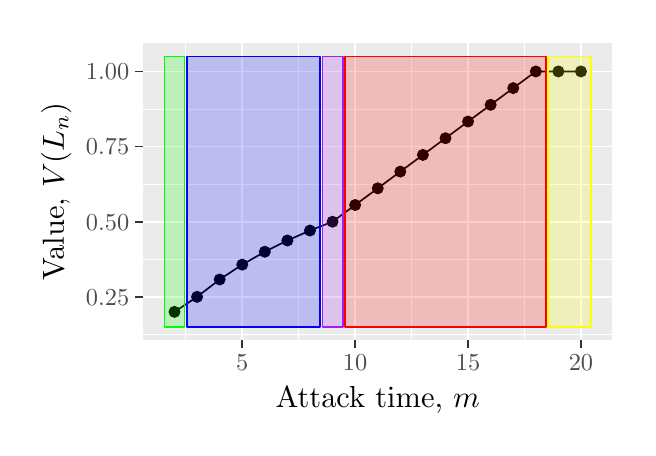
\begin{tikzpicture}[x=1pt,y=1pt]
\definecolor{fillColor}{RGB}{255,255,255}
\path[use as bounding box,fill=fillColor,fill opacity=0.00] (0,0) rectangle (216.81,144.54);
\begin{scope}
\path[clip] (  0.00,  0.00) rectangle (216.81,144.54);
\definecolor{drawColor}{RGB}{255,255,255}
\definecolor{fillColor}{RGB}{255,255,255}

\path[draw=drawColor,line width= 0.6pt,line join=round,line cap=round,fill=fillColor] (  0.00,  0.00) rectangle (216.81,144.54);
\end{scope}
\begin{scope}
\path[clip] ( 41.67, 31.53) rectangle (211.31,139.04);
\definecolor{fillColor}{gray}{0.92}

\path[fill=fillColor] ( 41.67, 31.53) rectangle (211.31,139.04);
\definecolor{drawColor}{RGB}{255,255,255}

\path[draw=drawColor,line width= 0.3pt,line join=round] ( 41.67, 33.70) --
	(211.31, 33.70);

\path[draw=drawColor,line width= 0.3pt,line join=round] ( 41.67, 60.85) --
	(211.31, 60.85);

\path[draw=drawColor,line width= 0.3pt,line join=round] ( 41.67, 88.00) --
	(211.31, 88.00);

\path[draw=drawColor,line width= 0.3pt,line join=round] ( 41.67,115.15) --
	(211.31,115.15);

\path[draw=drawColor,line width= 0.3pt,line join=round] ( 57.13, 31.53) --
	( 57.13,139.04);

\path[draw=drawColor,line width= 0.3pt,line join=round] ( 97.93, 31.53) --
	( 97.93,139.04);

\path[draw=drawColor,line width= 0.3pt,line join=round] (138.73, 31.53) --
	(138.73,139.04);

\path[draw=drawColor,line width= 0.3pt,line join=round] (179.53, 31.53) --
	(179.53,139.04);

\path[draw=drawColor,line width= 0.6pt,line join=round] ( 41.67, 47.28) --
	(211.31, 47.28);

\path[draw=drawColor,line width= 0.6pt,line join=round] ( 41.67, 74.43) --
	(211.31, 74.43);

\path[draw=drawColor,line width= 0.6pt,line join=round] ( 41.67,101.57) --
	(211.31,101.57);

\path[draw=drawColor,line width= 0.6pt,line join=round] ( 41.67,128.72) --
	(211.31,128.72);

\path[draw=drawColor,line width= 0.6pt,line join=round] ( 77.53, 31.53) --
	( 77.53,139.04);

\path[draw=drawColor,line width= 0.6pt,line join=round] (118.33, 31.53) --
	(118.33,139.04);

\path[draw=drawColor,line width= 0.6pt,line join=round] (159.13, 31.53) --
	(159.13,139.04);

\path[draw=drawColor,line width= 0.6pt,line join=round] (199.93, 31.53) --
	(199.93,139.04);
\definecolor{drawColor}{RGB}{0,0,0}
\definecolor{fillColor}{RGB}{0,0,0}

\path[draw=drawColor,line width= 0.4pt,line join=round,line cap=round,fill=fillColor] (191.77,128.72) circle (  1.96);

\path[draw=drawColor,line width= 0.4pt,line join=round,line cap=round,fill=fillColor] (199.93,128.72) circle (  1.96);

\path[draw=drawColor,line width= 0.4pt,line join=round,line cap=round,fill=fillColor] (118.33, 80.46) circle (  1.96);

\path[draw=drawColor,line width= 0.4pt,line join=round,line cap=round,fill=fillColor] (126.49, 86.49) circle (  1.96);

\path[draw=drawColor,line width= 0.4pt,line join=round,line cap=round,fill=fillColor] (134.65, 92.53) circle (  1.96);

\path[draw=drawColor,line width= 0.4pt,line join=round,line cap=round,fill=fillColor] (142.81, 98.56) circle (  1.96);

\path[draw=drawColor,line width= 0.4pt,line join=round,line cap=round,fill=fillColor] (150.97,104.59) circle (  1.96);

\path[draw=drawColor,line width= 0.4pt,line join=round,line cap=round,fill=fillColor] (159.13,110.62) circle (  1.96);

\path[draw=drawColor,line width= 0.4pt,line join=round,line cap=round,fill=fillColor] (167.29,116.66) circle (  1.96);

\path[draw=drawColor,line width= 0.4pt,line join=round,line cap=round,fill=fillColor] (175.45,122.69) circle (  1.96);

\path[draw=drawColor,line width= 0.4pt,line join=round,line cap=round,fill=fillColor] (183.61,128.72) circle (  1.96);

\path[draw=drawColor,line width= 0.4pt,line join=round,line cap=round,fill=fillColor] ( 53.05, 41.85) circle (  1.96);

\path[draw=drawColor,line width= 0.4pt,line join=round,line cap=round,fill=fillColor] (110.17, 74.43) circle (  1.96);

\path[draw=drawColor,line width= 0.4pt,line join=round,line cap=round,fill=fillColor] (102.01, 71.23) circle (  1.96);

\path[draw=drawColor,line width= 0.4pt,line join=round,line cap=round,fill=fillColor] ( 61.21, 47.28) circle (  1.96);

\path[draw=drawColor,line width= 0.4pt,line join=round,line cap=round,fill=fillColor] ( 69.37, 53.54) circle (  1.96);

\path[draw=drawColor,line width= 0.4pt,line join=round,line cap=round,fill=fillColor] ( 77.53, 58.91) circle (  1.96);

\path[draw=drawColor,line width= 0.4pt,line join=round,line cap=round,fill=fillColor] ( 85.69, 63.57) circle (  1.96);

\path[draw=drawColor,line width= 0.4pt,line join=round,line cap=round,fill=fillColor] ( 93.85, 67.64) circle (  1.96);

\path[draw=drawColor,line width= 0.6pt,line join=round] ( 53.05, 41.85) --
	( 61.21, 47.28) --
	( 69.37, 53.54) --
	( 77.53, 58.91) --
	( 85.69, 63.57) --
	( 93.85, 67.64) --
	(102.01, 71.23) --
	(110.17, 74.43) --
	(118.33, 80.46) --
	(126.49, 86.49) --
	(134.65, 92.53) --
	(142.81, 98.56) --
	(150.97,104.59) --
	(159.13,110.62) --
	(167.29,116.66) --
	(175.45,122.69) --
	(183.61,128.72) --
	(191.77,128.72) --
	(199.93,128.72);
\definecolor{drawColor}{RGB}{255,255,0}
\definecolor{fillColor}{RGB}{255,255,0}

\path[draw=drawColor,line width= 0.6pt,line join=round,fill=fillColor,fill opacity=0.20] (188.10, 36.42) rectangle (203.60,134.15);
\definecolor{drawColor}{RGB}{255,0,0}
\definecolor{fillColor}{RGB}{255,0,0}

\path[draw=drawColor,line width= 0.6pt,line join=round,fill=fillColor,fill opacity=0.20] (114.66, 36.42) rectangle (187.28,134.15);
\definecolor{drawColor}{RGB}{160,32,240}
\definecolor{fillColor}{RGB}{160,32,240}

\path[draw=drawColor,line width= 0.6pt,line join=round,fill=fillColor,fill opacity=0.20] (106.50, 36.42) rectangle (113.84,134.15);
\definecolor{drawColor}{RGB}{0,0,255}
\definecolor{fillColor}{RGB}{0,0,255}

\path[draw=drawColor,line width= 0.6pt,line join=round,fill=fillColor,fill opacity=0.20] ( 57.54, 36.42) rectangle (105.68,134.15);
\definecolor{drawColor}{RGB}{0,255,0}
\definecolor{fillColor}{RGB}{0,255,0}

\path[draw=drawColor,line width= 0.6pt,line join=round,fill=fillColor,fill opacity=0.20] ( 49.38, 36.42) rectangle ( 56.72,134.15);
\end{scope}
\begin{scope}
\path[clip] (  0.00,  0.00) rectangle (216.81,144.54);
\definecolor{drawColor}{gray}{0.30}

\node[text=drawColor,anchor=base east,inner sep=0pt, outer sep=0pt, scale=  0.88] at ( 36.72, 44.25) {0.25};

\node[text=drawColor,anchor=base east,inner sep=0pt, outer sep=0pt, scale=  0.88] at ( 36.72, 71.40) {0.50};

\node[text=drawColor,anchor=base east,inner sep=0pt, outer sep=0pt, scale=  0.88] at ( 36.72, 98.54) {0.75};

\node[text=drawColor,anchor=base east,inner sep=0pt, outer sep=0pt, scale=  0.88] at ( 36.72,125.69) {1.00};
\end{scope}
\begin{scope}
\path[clip] (  0.00,  0.00) rectangle (216.81,144.54);
\definecolor{drawColor}{gray}{0.20}

\path[draw=drawColor,line width= 0.6pt,line join=round] ( 38.92, 47.28) --
	( 41.67, 47.28);

\path[draw=drawColor,line width= 0.6pt,line join=round] ( 38.92, 74.43) --
	( 41.67, 74.43);

\path[draw=drawColor,line width= 0.6pt,line join=round] ( 38.92,101.57) --
	( 41.67,101.57);

\path[draw=drawColor,line width= 0.6pt,line join=round] ( 38.92,128.72) --
	( 41.67,128.72);
\end{scope}
\begin{scope}
\path[clip] (  0.00,  0.00) rectangle (216.81,144.54);
\definecolor{drawColor}{gray}{0.20}

\path[draw=drawColor,line width= 0.6pt,line join=round] ( 77.53, 28.78) --
	( 77.53, 31.53);

\path[draw=drawColor,line width= 0.6pt,line join=round] (118.33, 28.78) --
	(118.33, 31.53);

\path[draw=drawColor,line width= 0.6pt,line join=round] (159.13, 28.78) --
	(159.13, 31.53);

\path[draw=drawColor,line width= 0.6pt,line join=round] (199.93, 28.78) --
	(199.93, 31.53);
\end{scope}
\begin{scope}
\path[clip] (  0.00,  0.00) rectangle (216.81,144.54);
\definecolor{drawColor}{gray}{0.30}

\node[text=drawColor,anchor=base,inner sep=0pt, outer sep=0pt, scale=  0.88] at ( 77.53, 20.52) {5};

\node[text=drawColor,anchor=base,inner sep=0pt, outer sep=0pt, scale=  0.88] at (118.33, 20.52) {10};

\node[text=drawColor,anchor=base,inner sep=0pt, outer sep=0pt, scale=  0.88] at (159.13, 20.52) {15};

\node[text=drawColor,anchor=base,inner sep=0pt, outer sep=0pt, scale=  0.88] at (199.93, 20.52) {20};
\end{scope}
\begin{scope}
\path[clip] (  0.00,  0.00) rectangle (216.81,144.54);
\definecolor{drawColor}{RGB}{0,0,0}

\node[text=drawColor,anchor=base,inner sep=0pt, outer sep=0pt, scale=  1.10] at (126.49,  7.44) {Attack time, $m$};
\end{scope}
\begin{scope}
\path[clip] (  0.00,  0.00) rectangle (216.81,144.54);
\definecolor{drawColor}{RGB}{0,0,0}

\node[text=drawColor,rotate= 90.00,anchor=base,inner sep=0pt, outer sep=0pt, scale=  1.10] at ( 13.08, 85.29) {Value, $V(L_{n})$};
\end{scope}
\end{tikzpicture}
